% begin module continuity-ex1
\begin{frame}
\begin{example} %[Example 1, p. 113]
The picture below shows a graph of a function $f$.  \alert<handout:0 |2-3>{At which numbers is $f$ either discontinuous or not defined?}  \alert<handout:0 |4->{Why?}
\begin{columns}[c]
\column{.5\textwidth}
\begin{pspicture}(-0.5, -0.5)(5,6) \psframe*[linecolor=white](-0.5,-0.5)(5,6) \psaxes[ticks=x, labels=x]{<->}(0,0)(-0.5,-0.5)(5,6)
\psplot[linecolor=red, plotpoints=1000]{2}{5}{x 4 exp -0.0454545 mul x 3 exp 0.0555556 mul add x -1 mul add x 2 exp add 0.5 add }
\psplot[linecolor=red, plotpoints=1000]{-0.5}{2}{x 2 exp x 3 exp -0.5 mul add 1 add }
\psHollowDot{1}{1.5}
\psFullDot{2}{1}
\psHollowDot{2}{2.217171717}
\psHollowDot{4}{4.419191919}
\psFullDot{4}{2}
\end{pspicture}
%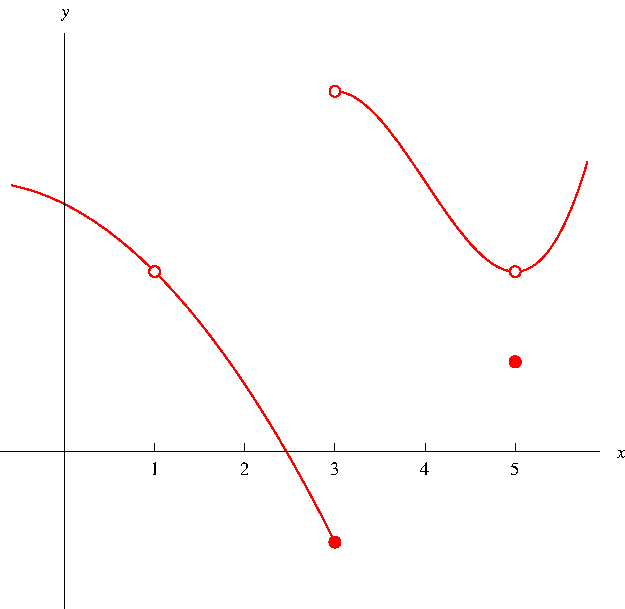
\includegraphics[height=4.5cm]{continuity/pictures/02-05-ex1.pdf}%

\column{.5\textwidth}
\begin{itemize}
\item<3->  Discontinuous at $1$:
\item<4->  \alert<handout:0 |5-6>{$\lim\limits_{x\rightarrow 1}f(x)$ \uncover<6->{exists.}}
\item<4->  \alert<handout:0 |7-8>{$f(1)$ \uncover<8->{is not defined.}}
\item<3->  Discontinuous at $2$:
\item<4->  \alert<handout:0 |9-10>{$f(2)$ \uncover<10->{is defined.}}
\item<4->  \alert<handout:0 |11-12>{$\lim\limits_{x\rightarrow 2}f(x)$ \uncover<12->{doesn't exist.}}
\item<3->  Discontinuous at $4$:
\item<4->  \alert<handout:0 |13-14>{$f(4)$ \uncover<14->{is defined.}}
\item<4->  \alert<handout:0 |15-16>{$\lim\limits_{x\rightarrow 4}f(x)$ \uncover<16->{exists.}}
\item<17-| alert@17>  $\lim\limits_{x\rightarrow 4}f(x) \neq f(4)$.
\end{itemize}
\end{columns}
\end{example}
\end{frame}
% end module continuity-ex1
